\section{Simulation Study}\label{sec:simulation}
\subsection{Setup}
In this section we will test the performance of the proposed $\QVP$ priors via a simulation study following the data-generating processes of \citet{bondell2010noncrossing}. 
%
We generate data from the following location scale heteroscedastic error model:
%
\begin{equation} \label{eq:loc-scale}
    y_t=\alpha_0+\beta^Tx_t+(\eta_0+\varrho^T_t \odot \eta_1^Tx_t)\varepsilon_t,~x_{t,k}\sim U(0,1),~\varepsilon_t\sim N(0,1).
\end{equation}
%
In total we consider the following 5 DGPs: 
%
\begin{itemize}
    \item $\mathrm{DGP}$-1: 4 predictors, with the $\beta_{\mathrm{DGP}_1}=\mathbbm{1}_K$, $\eta_1=0.1\mathbbm{1}_K$, and $\varrho_t=\mathbbm{1}_K$.
    \item $\mathrm{DGP}$-2: 10 predictors, with the parameters $\beta_{\mathrm{DGP}_2}=(\mathbbm{1}_4^T,\textbf{0}_6^T)^T$, $\eta_1=(0.1\mathbbm{1}_4^T,\textbf{0}_6^T)^T$, and $\varrho_t=\mathbbm{1}_K$.
    \item $\mathrm{DGP}$-3: 7 predictors, with the parameters $\beta_{\mathrm{DGP}_3}=\mathbbm{1}_k$, $\eta_1=(0.1\mathbbm{1}_3^T,\textbf{0}_4^T)^T$, and $\varrho_t=\mathbbm{1}_K$.
    \item $\mathrm{DGP}$-4: 10 predictors, with the parameters $\beta_{\mathrm{DGP}_4}=(\mathbbm{1}_4^T,\textbf{0}_6^T)^T$, $\eta_1=(0.1\mathbbm{1}_8^T,\textbf{0}_2^T)^T$, and $\varrho_t=(\mathbbm{1}_4^T,\mathbbm{1}_4^T  [I(\epsilon_t> F^{-1}_\varepsilon(0.9))+I(\epsilon_t\leq F^{-1}_\varepsilon(0.1))],\textbf{0}_2^T)^T$.%\tibi{Could you please be more explicit what you mean her by the t-subscript?}
    \footnote{Note that the $t$ subscript is needed since the presence of quantile variation will be dependent on the magnitude of $\varepsilon_t$.}
    \item $\mathrm{DGP}$-5: 4 predictors, with the parameters $\beta_{\mathrm{DGP}_5}=\mathbbm{1}_K$, $\eta_1=(0.1\mathbbm{1}_2^T,\mathbbm{1}_2^T)^T$, and $\varrho_t=\mathbbm{1}_K$.
\end{itemize}
%
%\tibi{I've added t subscripts to the $\varrho$s. I think this is correct? }
%
$\mathrm{DGP}$-1 and $\mathrm{DGP}$-2 are identical to the simulation study in \citet{bondell2010noncrossing}. $\mathrm{DGP}$-1 features non-zero location effects of the covariates, with a shallow but continuous upward slope in the quantile coefficient profile. $\mathrm{DGP}$-2 adds sparsity to the location where true zero coefficients do not display quantile variation. $\mathrm{DGP}$-3 is defined by non-zero location effects of the covariates, where only the first three coefficients have a shallow quantile profile. $\mathrm{DGP}$-4 adds to $\mathrm{DGP}$-3 extra covariates with true zero location and quantile varying effects. Additionally, 4 covariates display what \citet{kohns2021decoupling} call quantile specific sparsity patterns: location and quantile variation are zero for central quantiles, with large quantile variation in the extreme quantiles $\tau_q\geq0.9$ and $0.1\leq\tau_q$. $\mathrm{DGP}$-5 is generated with non-zero location effects, where for two covariates there is large continuous quantile variation. For ease of discussion below, we refer to coefficients of covariates with only location effects as quantile constant coefficients, to those coefficients with only a shallow profile $({\eta_1}_i = 0.1)$ as quantile varying coefficients, and those quantile varying coefficients with big jumps or large variation as extreme varying coefficients. %($\beta_{5:8}$ for $\mathrm{DGP}$-4 and $\beta_{3:4}$ for $\mathrm{DGP}$-5).
%

%
%$y_1$ and $y_2$ are identical to the ones in \citet{bondell2010noncrossing}. $y_1$ presents a case where every variable is important and portrays some quantile variation. $y_2$ is a DGP where only a subset of the variables are important, and these variables all portray quantile variation. $y_3$ is similar to that of \citet{bondell2010noncrossing}, but we keep quantile variation in $y_3$ to be the same as in $y_1$ and $y_2$. $y_4$ is a new cases: here we present a data generating process similar to $y_2$, but some of the covariates portray quantile varying sparsity as described in \citet{kohns2021decoupling}. We allow for the quantile varying sparse variables to have large impact at the tails. Finally, $y_5$ describes a data generating process similar to $y_1$, but half of the quantile varying variables portray large quantile variation.

%
We simulate sample sizes $\mathcal{T}=\{100,300\}$, and estimate models for various number of total quantiles $\mathcal{Q}=\{9,19,49\}$. We do this to address the fact that the $\QVP$ prior's shrinkage depends on how many quantiles are being estimated and because the previous literature warns of increasing probability of crossing quantile curves with many estimated quantiles \citep{jiang2013interquantile}. We allow the design matrix to be correlated with constant correlation of $\varDelta \in \{0, 0.5, 0.9\}$.\footnote{For $\varDelta>0$, the design is sampled form a normal distribution and then transformed using the min-max transformation on a column-wise basis.} We generate $N_{\mathrm{sim}} = 500$ simulated data sets. For posterior inference we obtain per model 25000 MCMC draws for 4 chains in parallel, of which we discard the first 10000 each as burnin.  %We opt to do this because it is unlikely that applied datasets will have no correlation in the design matrix.
%

Recovery of $\boldsymbol{\beta}$ is measured based on the root-mean-squared-error for the i\textsuperscript{th} DGP, by $\mathrm{RMSE}_i$:
%
\begin{equation} \label{eq:rmse_def}
    \mathrm{RMSE}_i =  \sqrt{\frac{1}{N_{\mathrm{sim}}\mathcal{Q}}\sum_{j = 1}^{N_{\mathrm{sim}}}\sum_{k=1}^{K_{\mathrm{DGP}_{i}}} \sum_{q=1}^{\mathcal{Q}} \left( {\beta_{k,q}} - {{\hat{\beta}_{j,k,q}}} \right)^2},
\end{equation}
%
where $\beta_{k,q}$ is the DGP's true coefficient at the $q$\textsuperscript{th} quantile and $\hat{\boldsymbol{\beta}}$ refers to the posterior mean defined as: 
\begin{equation}
    \begin{split}
        \hat{\boldsymbol{\beta}} = \E{\boldsymbol{\beta}|y} &  = \int_{\mathbbm{R}^{\mathcal{Q}K}}\boldsymbol{\beta} \; p(\boldsymbol{\beta}|y)\;\mathrm{d}\boldsymbol{\beta} \\
        & \approx \frac{1}{S}\sum_{s = 1}^S \boldsymbol{\beta}^{(s)}.
    \end{split}
\end{equation}
%
Denote the $q\textsuperscript{th}$ fitted quantile for observation $t$ based on the posterior mean as $\hat{Q}_{\tau_q,t}$. We evaluate predictions with the Quantile score ($\mathrm{QS}_{q,i}$) for the q\textsuperscript{th} quantile and i\textsuperscript{th} DGP:
%
\begin{equation}
    \mathrm{QS}_{\tau_q,i} =  \frac{1}{N_{\mathrm{sim}}}\sum_{j = 1}^{N_{\mathrm{sim}}} \frac{1}{T}\sum^\mathcal{T}_{t=1}\rho_{\tau_q}\left( {y_{j,t}} - \hat{Q}_{j,\tau_q,t} \right)
\end{equation}
%
The $\mathrm{QS}$ score belongs to the strictly proper scoring rules \citep{gneiting_strictly_2007} calculated for every simulation run based on 100 independently generated out of sample observations. The $\mathrm{QS}$ may be used to evaluate different combinations of quantiles to get an idea of the performance at different parts of the predictive density. To achieve this, we will follow \citet{gneiting2011comparing} in calculating the quantile weighted $\mathrm{QS}$:

\begin{equation}\label{eq:qwQS}
    \mathrm{qwQS}_i = w_{\tau_q} \mathrm{QS}_{i,\tau_q}%d\tau_q,
\end{equation}

\noindent where $w_{\tau_q}$ denotes a weighting scheme. We consider four different weighting schemes: (a) $w_{\tau_q}^1=\frac{1}{Q}$ places equal weight on all quantiles, which is equivalent to taking an average of the weighted residuals; (b) $w_{\tau_q}^2={\tau_q}(1-{\tau_q})$ places more weight on central quantiles; (c) $w_{\tau_q}^3=(1-{\tau_q})^2$ places more weight on the left tail; and (d) $w_{\tau_q}^4={\tau_q}^2$ places more weight on the right tail.  
%, which we evaluate for $\dotsc$
%\tibi{Please adjust as you think it makes sense to further define the quantile score.}
%

Lastly, we measure the incidence of crossing. The crossing incidence is calculated by comparing the fitted quantiles with the sorted quantiles following the procedure of \citet{chernozhukov2010quantile}:

\begin{equation}\label{eq:cross-i}
    \mathrm{Cross}_{\tau_q,i}=\frac{1}{N_{\mathrm{sim}}} \sum_{j =1}^{N_{sim}} \frac{1}{\mathcal{Q}\mathcal{T}}\sum^{\mathcal{T}}_{t=1}\sum^{\mathcal{Q}}_{q=1}I[{\hat{Q}_{{j,\tau_q,t}}\neq\hat{Q}^{\mathrm{sort}}_{{j,\tau_q,t}}}],
\end{equation}

\noindent where $\hat{Q}^{\mathrm{sort}}_{{\tau_q,t}}$ is the sorted predicted quantile. The crossing incidence measures the proportion of quantiles that need sorting after estimation to adhere to the property of monotone quantile functions. The lower the $\mathrm{Cross}$ value, the less quantiles need to be rearranged after estimation.% 

Next to the $\QVP$, $\NCQVP$, $\NCQVP_{\mathrm{SAVS}}$, we consider two approaches for independent Bayesian quantile regression, the $\BQR$ as presented in \citet{kozumi2011gibbs} with flat priors and the $\HSBQR$ of \citet{kohns2024horseshoe} which uses horseshoe priors on the quantile coefficients, respectively. 
Since both assume that the quantile functions are unrelated, we refer to these as independent quantile regression methods. We expect the independent quantile methods to do well for $\mathrm{DGP}$-4 where quantile specific sparsity is present. Additionally, to illustrate the benefit of estimating the quantile profile $\beta_q$ in addition to the composite quantile vector $\beta_0$, we also estimate a Bayesian composite quantile model which only models $\beta_0$, the $\mathrm{CQR}$ model. 
%
Lastly, since the QVP prior is motivated from the non-crossing quantile objective function of \citet{bondell2010noncrossing}, we include their model too for comparison, denoted $\BRW$.
%as a competitor to the Bayesian approach, we consider the non-crossing adaptive lasso estimator of \citet{bondell2010noncrossing}, $\mathrm{BRW}$. \dk{make sure that the acronyms are formatted the same throughout}.
\subsection{Results}
\subsubsection{Coefficient Recovery}
%
\begin{figure}
    \centering
    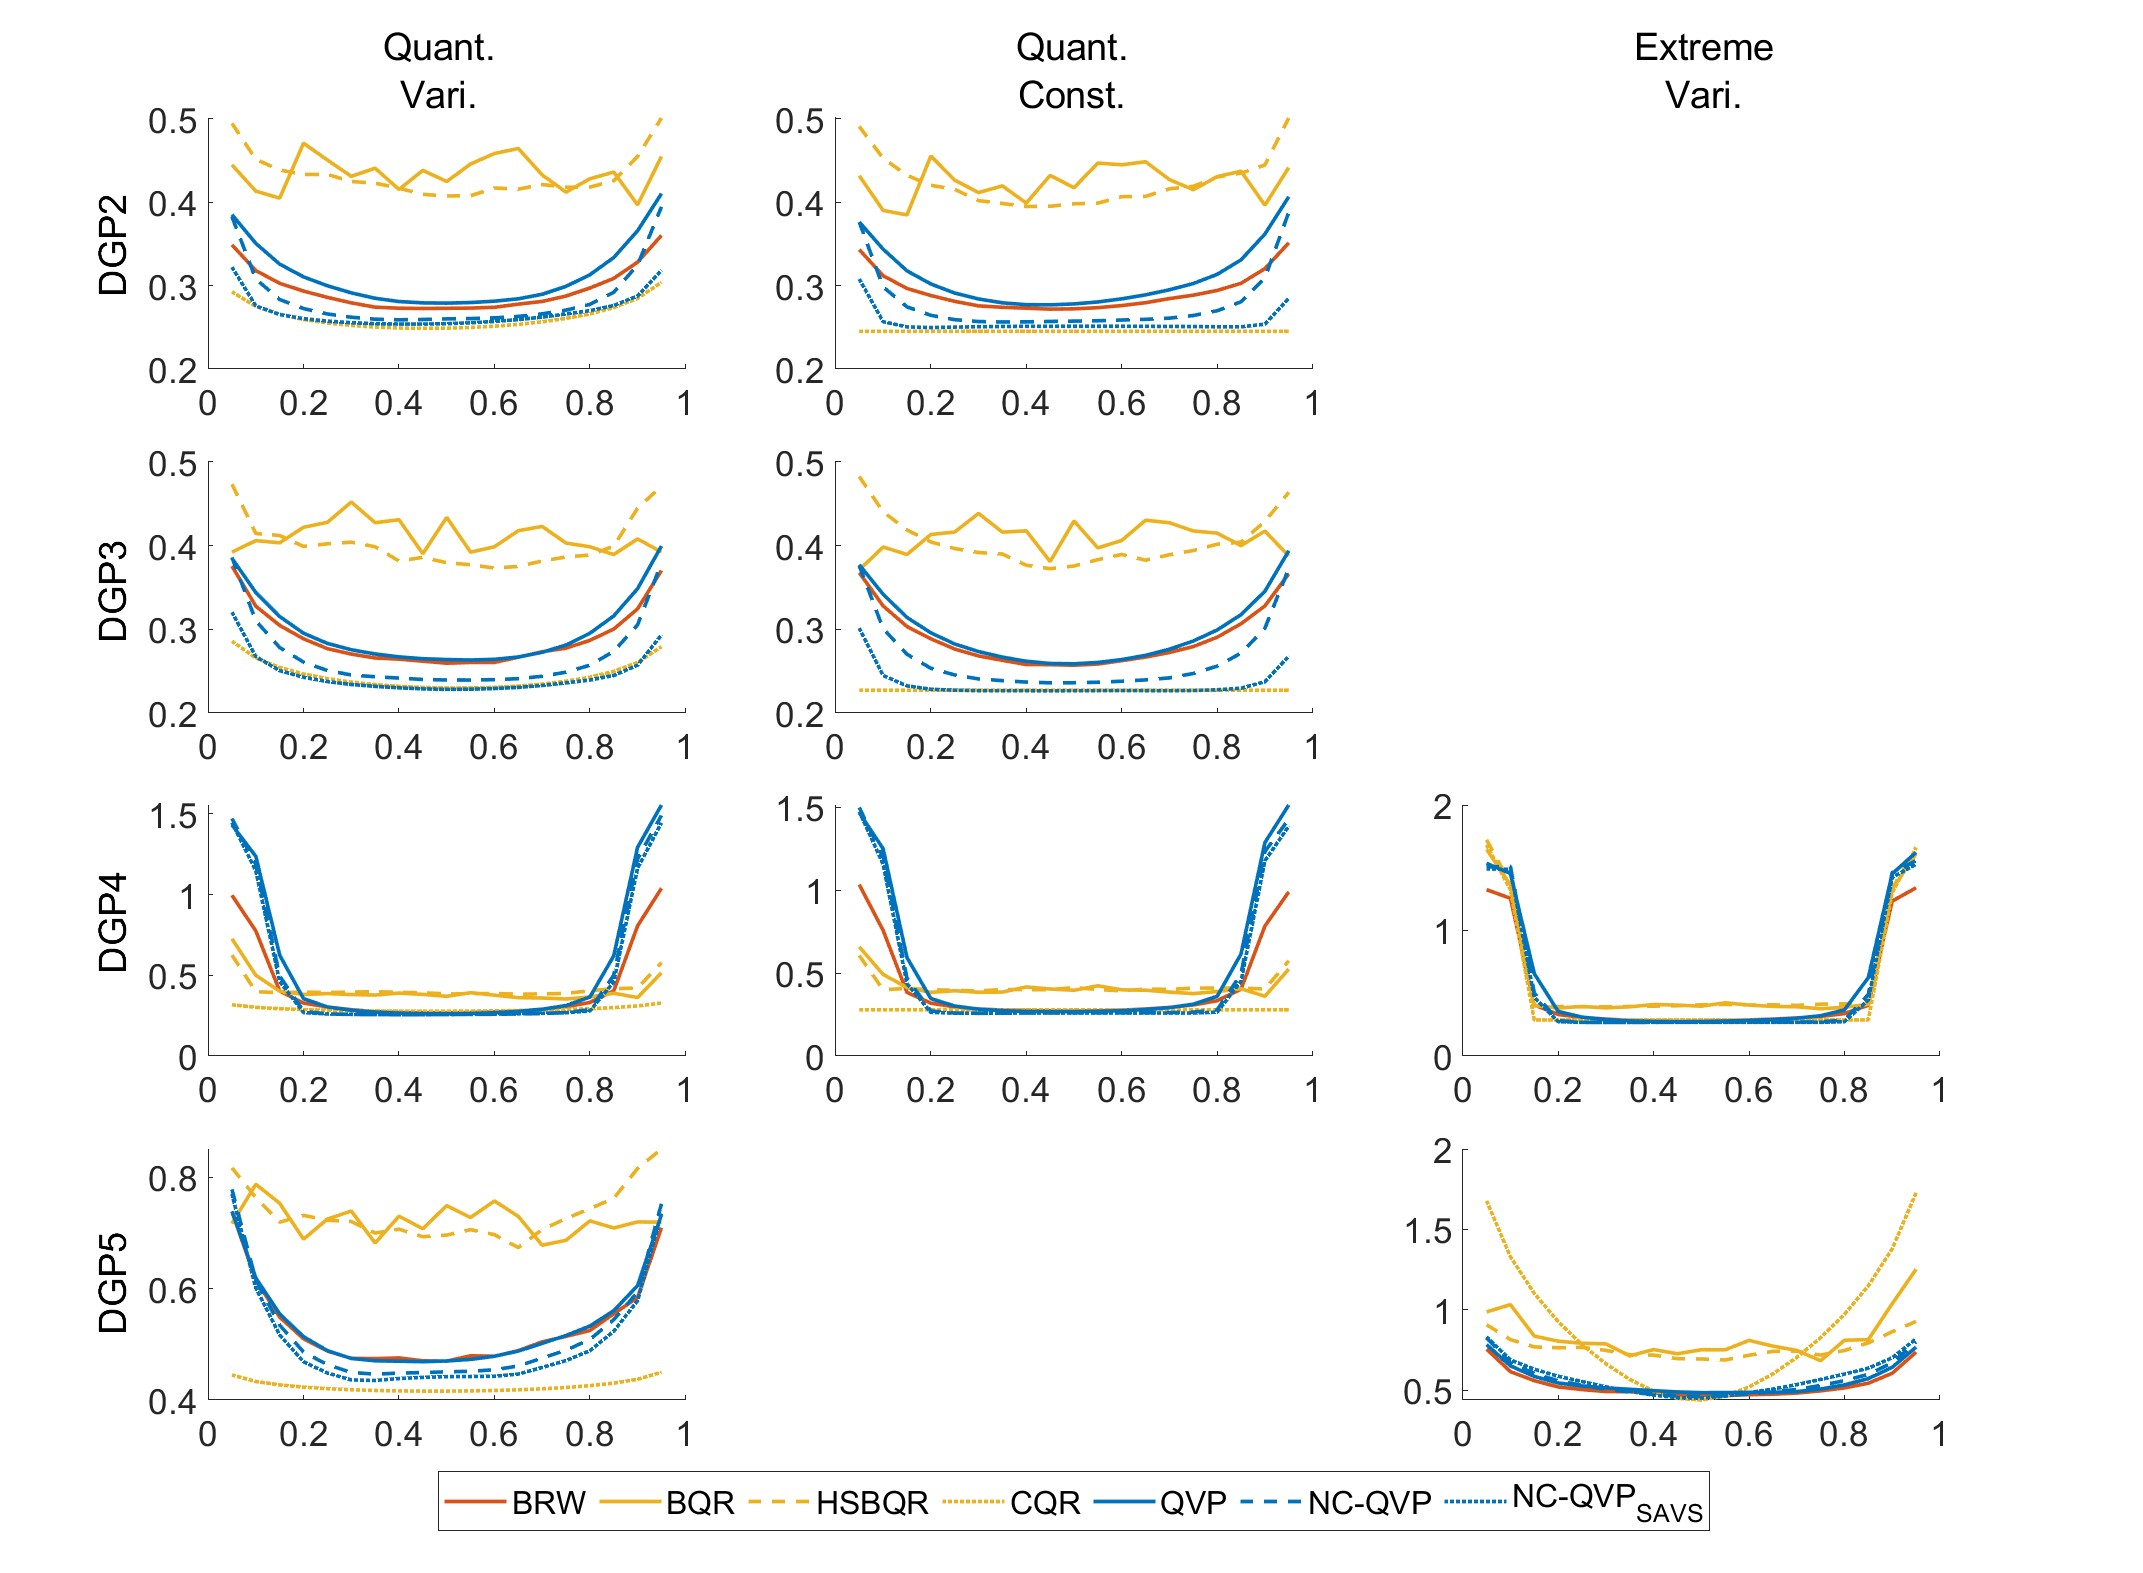
\includegraphics[width=\linewidth]{Figures/CoeffBiasSpecificv3.jpg}
    \caption{$\rmse$ profile of $\boldsymbol{\beta}$ across 19 quantiles $\tau_q \in \left\{0.05,\dotsc,0.95\right\}$ for $\mathcal{T}=300$ and $\varDelta$=0. Estimates are based on the posterior mean. }
    \label{fig:SpecCoeffBias}
\end{figure}
%
We summarise coefficient recovery in Figure~\ref{fig:SpecCoeffBias} for $\mathcal{T}=300$ and $\mathcal{Q}=19$ estimated quantiles. In Figures~\ref{fig:C4} and~\ref{fig:C5}, we additionally show estimated coefficient profiles for a variable with quantile specific sparsity for $\mathrm{DGP}$-4 and large quantile variation for $\mathrm{DGP}$-5 respectively.\footnote{See  Appendix~\ref{app:extra-sim-results} for figures also for coefficients the other DGPs.} See Appendix~\ref{app-sec:fig-posteriors} for average performance for the central and extreme quantiles for the different permutations of $(T,\varDelta)$. 
%

As expected, Figure~\ref{fig:SpecCoeffBias} shows that the $\NCQVP$ and $\CQR$ models perform generally best for coefficients with low quantile variation or no quantile vairation at all (columns 1 and 2), particularly visible for DGPs 2-3. The $\mathrm{CQR}$ does well for these DGPs because estimating the true shallow quantile profile to be zero only causes small increases in $\mathrm{RMSE}$. $\NCQVP$ and $\NCQVP_{\mathrm{SAVS}}$ shrink low quantile variation heavily to zero, and therefore perform for these DGPs well, too. In fact the SAVS variant is on par with the $\mathrm{CQR}$ model. %Hence, the extra shrinkage and sparsification by the non-centred parameterisation is able to recover low quantile variation. 
The $\NCQVP$ offers not only a large improvement over methods that estimate the quantiles independently ($\BQR$,$\HSBQR$), but it also clearly outperforms $\mathrm{BRW}$. This is particularly visible for the quantile constant coefficients of the $\mathrm{DGP}$-3, in which the true constant coefficients are non-zero. In line with the motivation of the $\QVP$ prior's structure, we find that for $\mathrm{DGP}$-2-3, it generally performs on par with the $\mathrm{BRW}$. 
%

For $\mathrm{DGP}$-4 in which there is pronounced quantile specific sparsity, we see that that  models which do not explicitly model the difference in quantile coefficients ($\BQR$, $\HSBQR$, $\CQR$) may outperform the $\QVP$ models. However, Figure~\ref{fig:C4} shows that these models also falsely shrink away the true profile to zero in the extreme tails. The $\QVP$ models, in contrast, correctly recover the coefficient profile, albeit with larger variance in the tails. With increasing number of observations, we would expect the reduction in posterior variance to lead also to superior $\mathrm{RMSE}$ for the $\QVP$ models over the independent quantile methods.
%

For coefficients that showcase large continuous variation across all quantiles, $\mathrm{DGP}$-4 and $\mathrm{DGP}$-5 (column 3 of Figure~\ref{fig:SpecCoeffBias}), we can see that recovery of the $\mathrm{QVP}$ models is competitive in terms of RMSE (Figure~\ref{fig:SpecCoeffBias}) and estimated coefficient profile (Figure~\ref{fig:C5}). As expected, the $\mathrm{QVP}$ model tends to outperform the $\NCQVP$ here since less shrinkage on the difference between quantiles is exerted in the centred formulation. The uncertainty bands compared to independent estimation of the quantiles, indicates large efficiency benefits to joint estimation. 
%

These findings are robust to the number of data points (Appendix, Figure~\ref{fig:SpecCoeffBias_T100}), magnitude of correlation between covariates (Appendix, Figures~\ref{fig:SpecCoeffBias_rho05} and \ref{fig:SpecCoeffBias_rho09}), the number of quantiles estimated (Appendix, Figures~\ref{fig:SpecCoeffBias_Q9} and \ref{fig:SpecCoeffBias_Q39}) and from the perspective of predictive performance (Appendix, Section~\ref{app:sims-predictive-results}). In fact, with more quantiles estimated, we find that there are further performance gains with the $\QVP$ compared to the $\NCQVP$ in $\mathrm{DGP}$-5. Here, less shrinkage of the coefficient profile with the $\QVP$ over the $\NCQVP$ allows for improved modelling in the tails with the finer resolution offered by modelling more quantiles.  
%

Hence, in terms of parameter recovery, the $\QVP$ framework provides an excellent balance between the composite quantile model that only models location effects and the $\BRW$ model which strictly enforces non-crossing. The $\NCQVP$ model in particular benefits from stronger between-quantile shrinkage when little quantile variation is present, yet also does not overtly shrink true large variation in quantile profiles. To choose in practice between the centred and non-centred formulation, we recommend using the $\NCQVP$ as the baseline with which to test for the presence of no quantile variation with the $\mathrm{SAVS}$ algorithm. If significant quantile variation is present, then we recommend using the $\QVP$ model.%\dk{Not sure about this one, let me know what you think}.
\footnote{We leave investigation in terms of model selection properties for future research.} Despite the relatively low dimensionality of the covariate set, the DGPs show that the QVP methods are always preferable to independent quantile models.
%
\begin{figure}
    \centering
    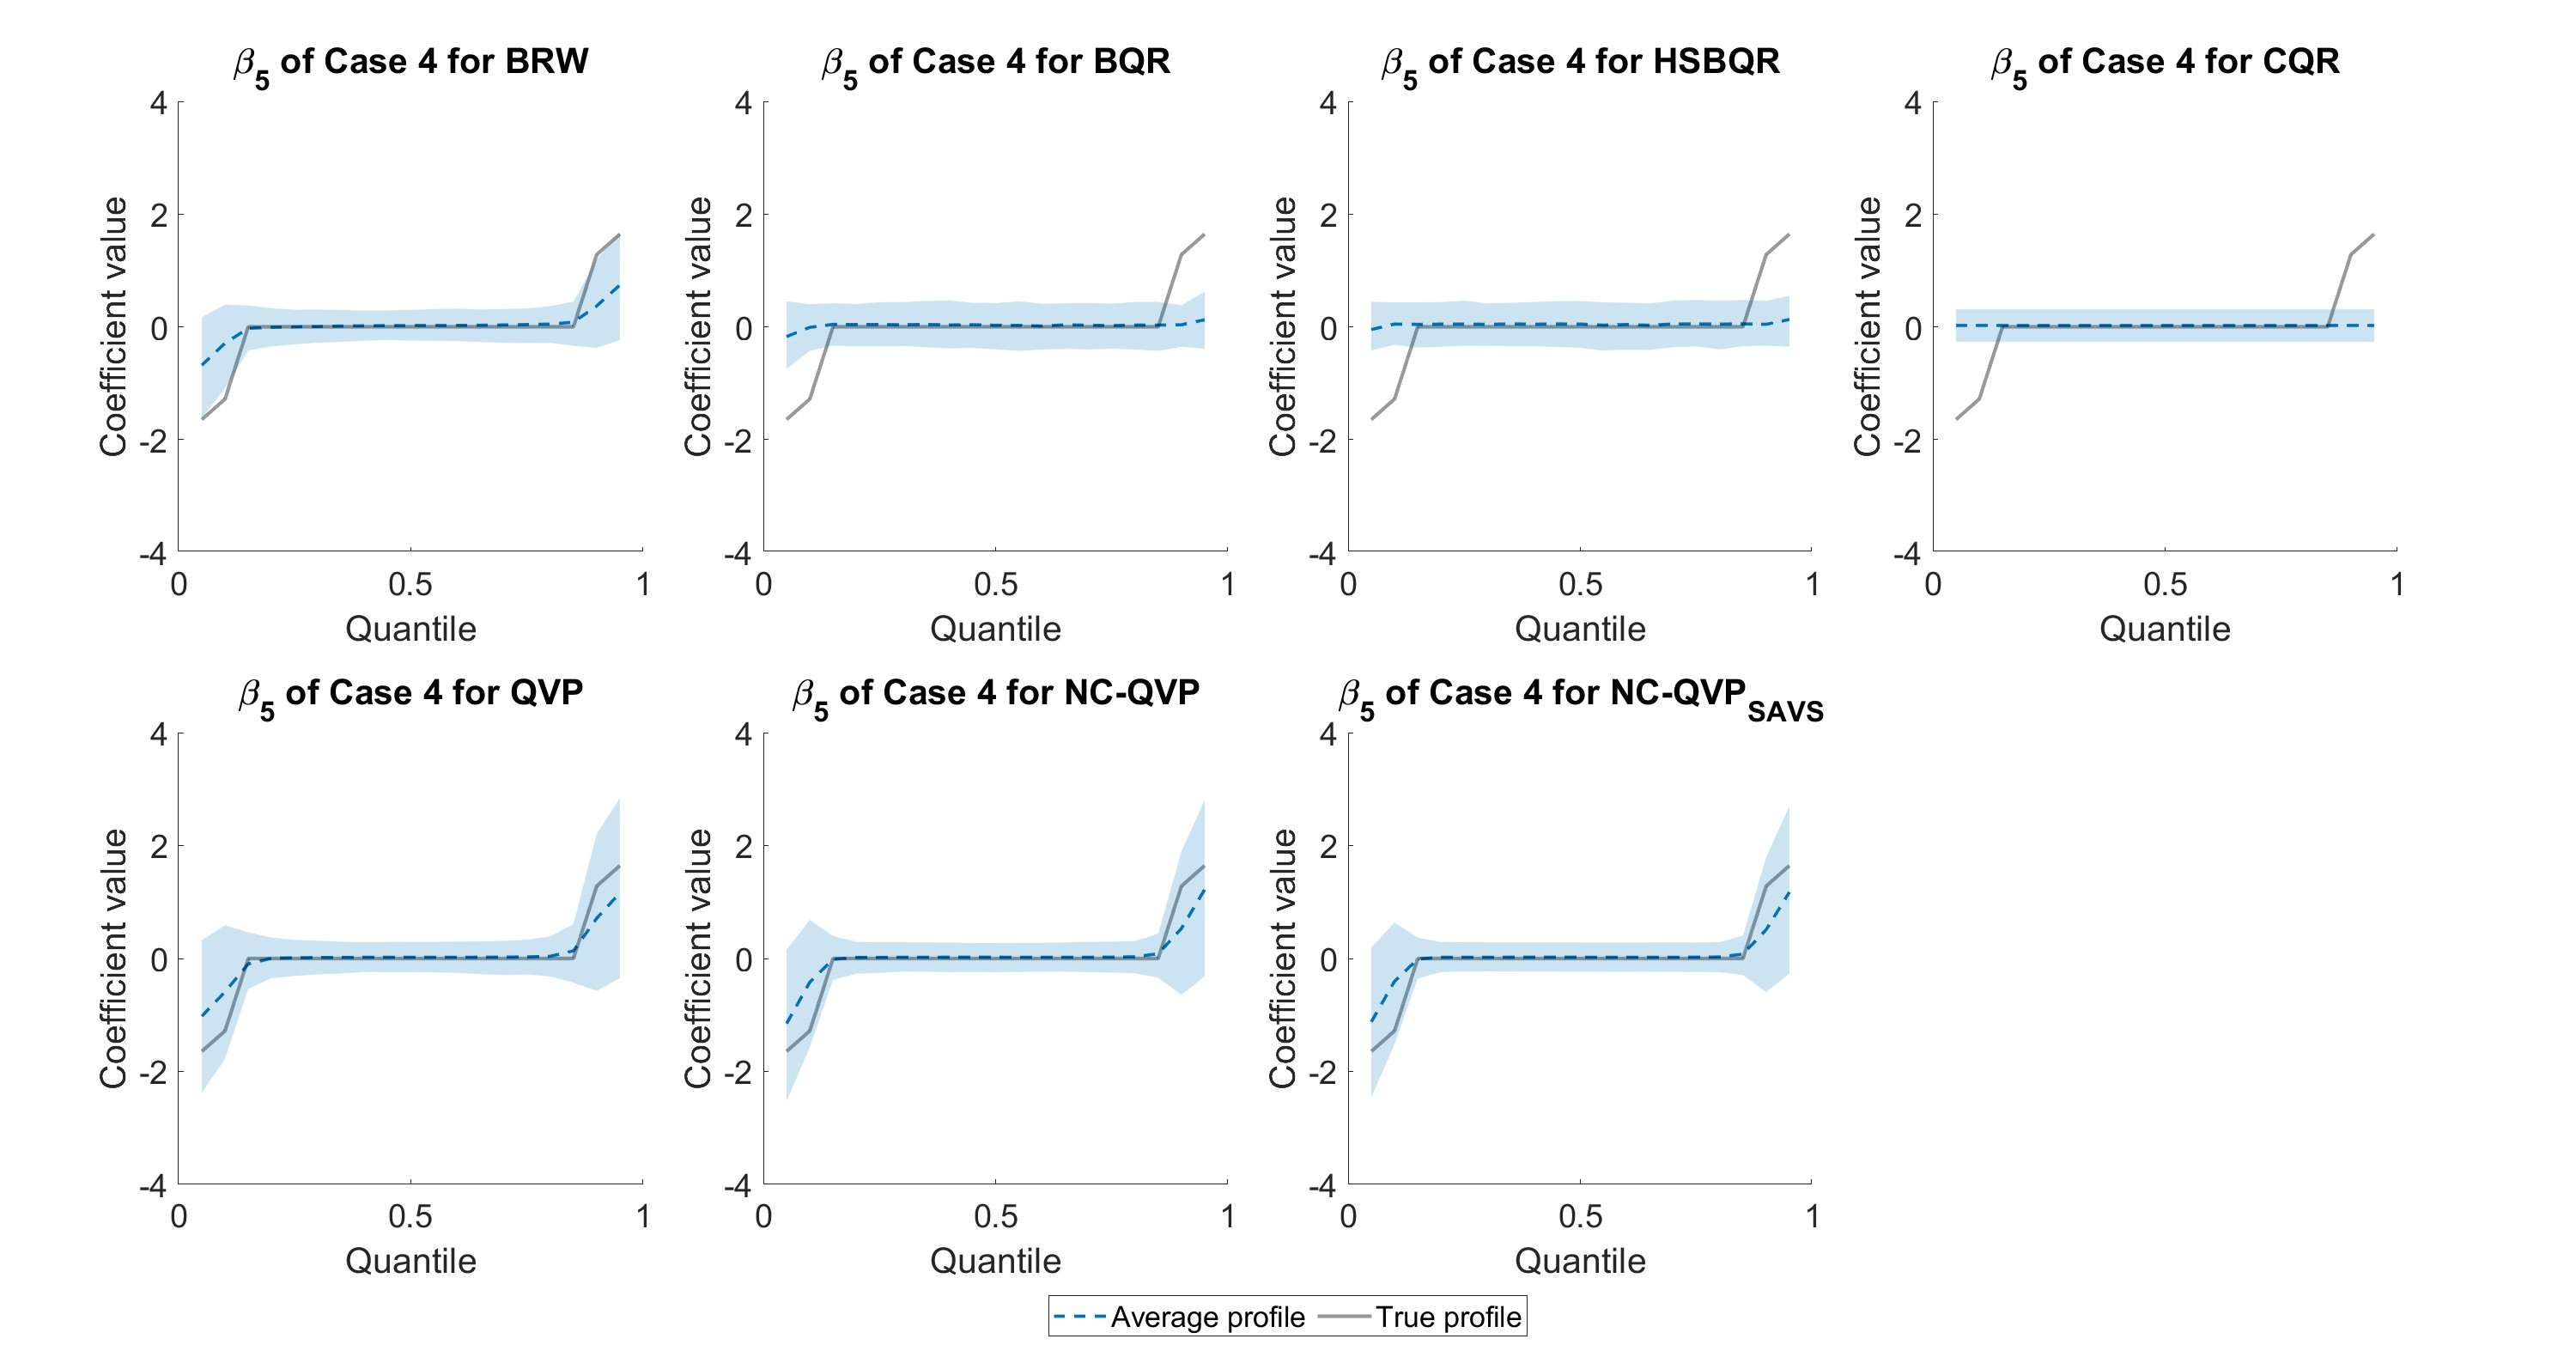
\includegraphics[width=\linewidth]{Figures/PresFig4_T=300.jpg}
    \caption{Coefficient posterior for $\mathrm{DGP}$-4, $\mathcal{T}=300$, $\varDelta$=0. Dotted lines show the average of the posterior means. The blue area reprents the central 95$\%$ interval of the posterior means.} %the blue area represent width of standard error around the posterior mean. 
    \label{fig:C4}
\end{figure}

\begin{figure}[h]
    \centering
    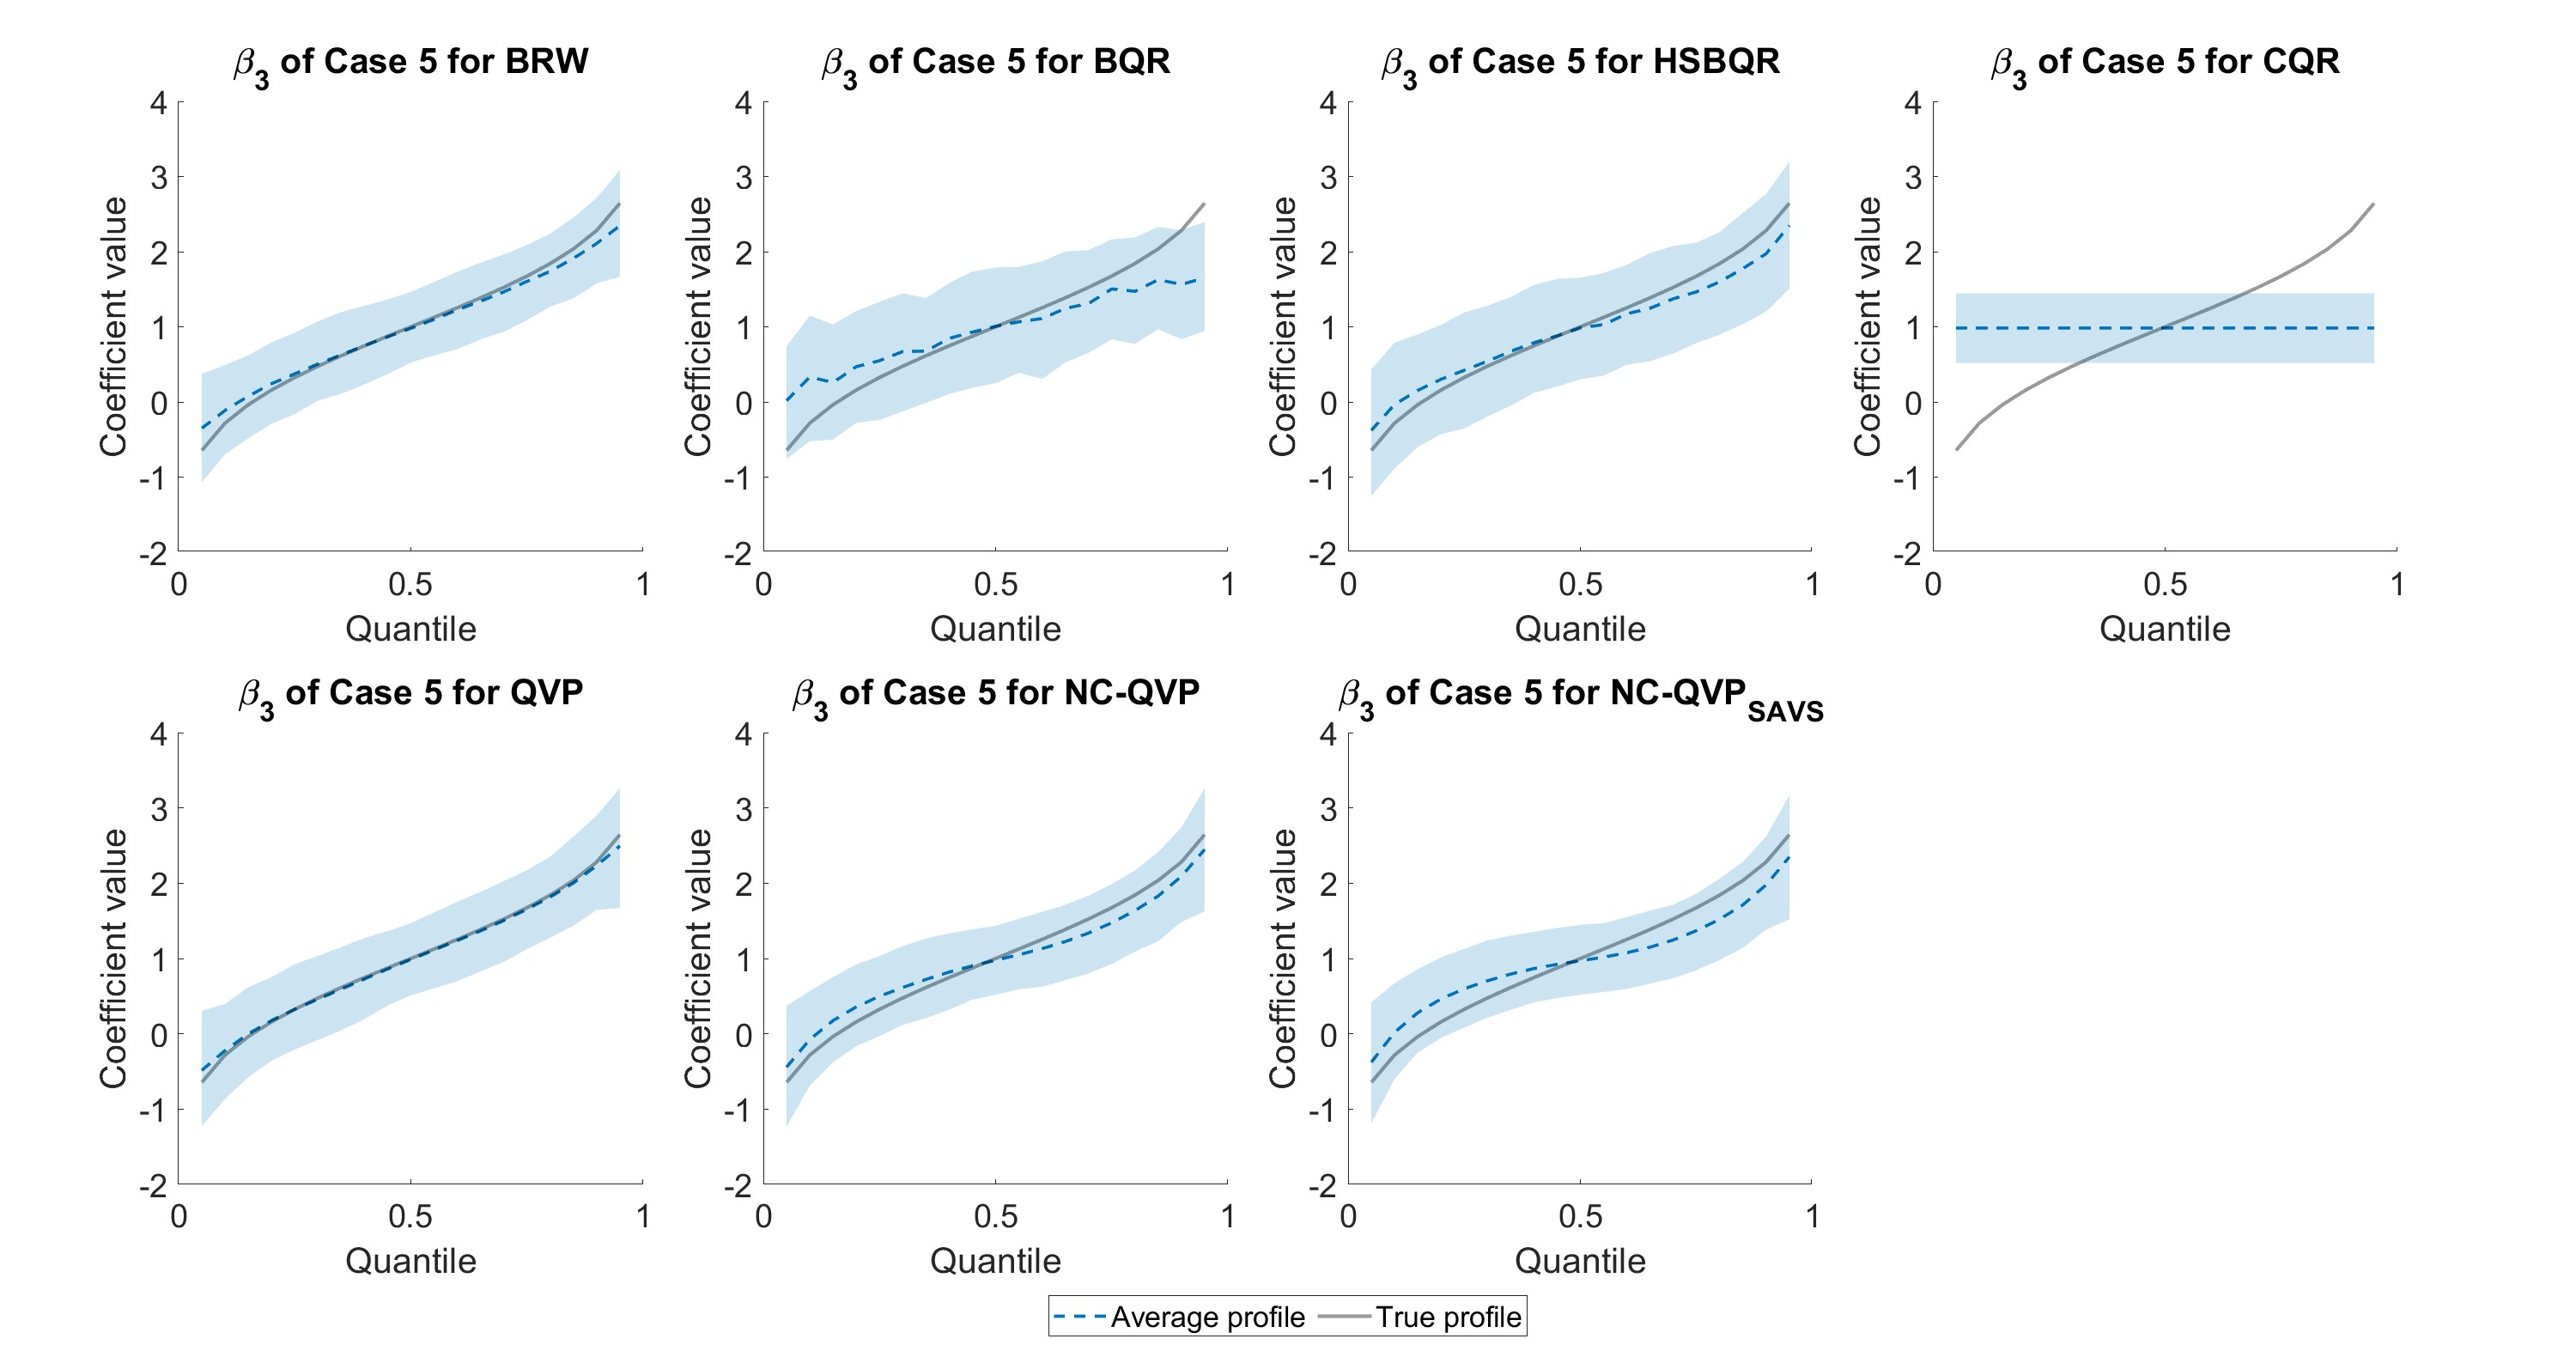
\includegraphics[width=\linewidth]{Figures/PresFig3_T=300.jpg}
    \caption{Coefficient posterior for $\mathrm{DGP}$-5, $\mathcal{T}=300$, $\varDelta$=0. Dotted lines show the average of the posterior means. The blue area reprents the central 95$\%$ interval of the posterior means.}
    \label{fig:C5}
\end{figure} 
%
\subsubsection{Robustness}
The improvements in parameter recovery of the $\mathrm{QVP}$ models also translate to a lower incidence of crossing fitted quantiles as well as improved sampling efficiency. Table~\ref{tab:cross} shows that independent of the simulation design, the $\mathrm{QVP}$ models almost completely eliminate crossing. Hence, free estimation of the implied non-crossing penalty parameter on the differences across quantiles (compare Equation~\ref{eq:fused-objective-function}), is sufficient to regularise the posterior toward the desired area of non-crossing. Independent quantile models struggle comparatively more with $\mathrm{DGP}$~1 and $\mathrm{DGP}$~2, where separation of quantile varying and non-varying coefficients is complicated by the relatively low amount of cross-quantile variation. 
%

Figure~\ref{fig:RobustMeas} shows that for all $\mathrm{DGP}$s, the $\QVP$ models' $\hat{R}$ and effective sample size, $\mathrm{N}_{\mathrm{eff}}$ of \citet{vehtari2021rank} indicate good mixing, as well as large efficiency gains of the $\mathrm{MCMC}$ sampler over the $\BQR$ and $\HSBQR$ models. As expected, sampling is more efficient for the $\mathrm{QVP}$ model for $\mathrm{DGP}$-5 due to the large quantile variation. 

%\dk{old from here}
%The coefficient bias results for the different Monte Carlo experiments are shown in table (\ref{tab:overallbias_main}). While we estimate every $5^{th}$ (Q=19) quantile, we only show the coefficient bias at the 10th, 50th and 90th quantile. In this table we show the case when the covariates are not correlated. The values for the BQR are the raw coefficient bias, while every other estimator's value is relative the BQR's value. In this way we can see which estimators yield gains above the BQR at a glance. In table (\ref{tab:overallbias_quant}) we produce the same table for rho=0.0, and T=300, but varying the number of quantiles to every $10^{th}$ (Q=9) and every $2.5^{th}$ (Q=39). Since joint estimation depends on the number of quantiles being estimated we wish to see how sensitive the method is to varying the number of quantiles. Finally, in the appendix (table (\ref{tab:overallbias_rhos})) we also produce a table (for Q=19), for the case when the covariates are correlated.

%The tables reveal that joint esitmation of the quantiles always yields lower coefficient bias than individually estimating the quantiles: BRW and the QVP priors consistently have lower coefficient bias than the BQR and HSBQR.

%The second observation is that for case 4 all the estimators struggle at the tails. Surprisingly, the BQR and HSBQR also have difficulty with quantile specific sparse setting, even though this specification is biased towards independent estimation of the quantiles. Interestingly, the estimators that jointly estimate all quantiles perform better than the independent quantile estimators at the median for this case.

%When looking at the overall performance of the joint estimators, we can see that the QVP prior performs about as well as the BRW estimator. Importantly, we show that our NCQVP variants can yield further improvements, with all NCQVP variants having lower coefficient bias than the BRW for almost all cases, except case 4. %Furthermore, the ASIS variants of the NCQVP perform particularly well for cases 2, 3, and 5. These are the cases where there are quantile constant and quantile varying variables present, i.e. the cases where there is a variable selection needed in the fused setting.

%omparing the QVP prior to the CQR highlights how one can obtain lower coefficient bias results for the small quantile varying cases 1 and 2. The table shows that for larger quantile variation, the performance of the CQR suffers greatly compared to the NCQVP variants. Importantly, the difference between the NCQVP and the CQR for the small quantile varying cases is small. The advantage of the QVP prior is that it is able to adapt to the degree of quantile variation: it has better performance than the CQR for large quantile variation cases, while it does not do much worse than CQR for small quantile varying cases. This adaptability is important in applied settings, as practitioners rarely know the degree of quantile variation in a database ex-ante.

%Adding SAVS to the quantile difference part of the NCQVP setup yields further improvements: we can see that in all cases including SAVS helps with overall coefficient bias for all the cases considered. While we would expect SAVS to help for cases 2,3,4, and 5 on account of quantile constant variables being present, it is surprising that SAVS leads to overall lower coefficient bias for case 1 as well.

%These results carry over to T=300 case where we can see that the QVP prior variants lead to gains over the traditional estimators. Importantly, some of the NCQVP variants yield coefficient bias results for T=100, that are lower than the independent quantile estimators with T=300, e.g. NCQVP with SAVS in case 1. %This is particularly impressive and showcases the power of the NCQVP framework. 

%\tibi{PLACEHOLDERS PARAGRAPHS FOR NOW}
%\tibi{Varying the number of quantiles in table (\ref{tab:overallbias_quant}), has no impact on the BQR estimator, as expected. The same can not to be said for the joint estimator methods, where Q=39 has less gains than Q=9, for most cases considered. The only exception is Case 5, where estimating more quantiles leads to further improvements in coefficient bias for the joint estimators. This highlights, that if there is large degree of quantile variation in some of the variables, estimating more quantiles can help recover the true quantile profile.}

%\tibi{Table (\ref{tab:overallbias_rhos}) shows the coefficient bias results for the different settings when the covariates are correlated to different degrees. We note that the coefficient bias results are higher for all the estimators compared to their uncorrelated variants. However, the relative performance of the QVP prior, with the NCQVP framework in particular, remains: the proposed estimators comfortable lead to lower coefficient bias than the independent quantile estimators. Furthermore, the NCQVP framework leads to further gains, leading to lower coefficient bias than the BRW.}


%
%Figure (\ref{fig:SpecCoeffBias}) shows the coefficient bias for the different types of variables. The top block shows the coefficient bias for the constant, the next block shows the coefficient bias for the (small) quantile varying variable. The following block is the quantile constant variables coefficient bias. The final block in the figure is the case specific variables, i.e. quantile specific sparse variables for case 4, and large quantile variation for case 5.

%From the figure we can see that jointly estimating the quantiles almost always leads to lower coefficient bias than independently estimating the quantiles. The only case where this is not the case is for case 4, the quantile specific sparse case, which is a data generating process that is biased towards the independent quantile estimators. Furthermore, we can also see that the NCQVP framework often leads to lower coefficient bias in the constant than the BRW estimator, except for case 4 but even here the NCQVP framework performs about as well as the BRW.

%When looking at the quantile varying variables, we can see again that the estimators that jointly estimate the quantiles fare better. While most estimators perform about as well as the BRW, we again see that the NCQVP framework has gains as it often leads to lower coefficient bias than the BRW estimator with the only exception being case 4.

%The quantile constant variables are particularly interesting since the fused shrinkage framework is meant to help us identify the variables that vary by quantile. Here we can see gains for all joint estimation frameworks, but again the NCQVP is particularly potent often yielding lower coefficient biases than the BRW. Furthermore, we can see that the SAVS variant of the NCQVP lead to large gains in the quantile constant and quantile varying variables. As such, putting SAVS on the estimators helps in identifying quantile constant variables and shrinking their quantile variation to 0. This in turn helps with identifying, and correctly estimating the size, of the coefficients of the quantile varying variables.

%When looking at the case specific variables we can see again that for case 4 the QVP prior methods struggle compared to the independent quantile estimators. %However, the ASIS variants of the NCQVP framework yields coefficient biases that are close to the independent quantile estimators. 
%Surprisingly the BRW estimator has the lowest coefficient bias for the quantile specific sparse variables. For case 5 with the large quantile varying variables the QVP prior again show large gains, leading to the lowest coefficient biases. %Interestingly, the SAVS variant of the NCQVP with ASIS has worse coefficient bias than the estimator without SAVS. This shows that implementing SAVS does not often lead to gains in estimation. 

%The figure also gives insight into where the gains of the CQR are from: constraining the quantile variation to be 0 helps in identifying the $\beta_0$. When quantile variation is small, this gain outweighs the loss at the performance in the tails. However, when quantile variation is large, as it is in case 5, the CQRs performance become noticably worse for the coefficients that vary by a lot.


%Overall, we see that the QVP framework, and the NCQVP in particular, leads to lower coefficient bias for almost all cases. We can also glean from the more detailed breakdown that this improvement comes from being able to distinguish between quantile constant (and quantile varying) variables. %Furthermore, we can see that the ASIS variants lead to gains in performance when there is quantile specific sparsity, or when the degree of quantile variation is large. 
%The results also show the problems of estimating quantile specific sparse models, and this highlights that although joint estimation is potent, it is not a panacea to all quantile estimation problems.


%\subsubsection{Robustness measures and crossing incidence}
%Figure (\ref{fig:RobustMeas}) shows the Rhat and effective independent samples (Neff) for all the bayesian estimators. When looking at the Rhat of the various bayesian estimators, we can see that the joint estimation frameworks do not have any difficulties in convergence of the MCMC chains. In particular we can see that the Rhat is well below even 1.01 for all cases.

%When looking at effective independent samples of the Bayesian estimators, we can see that the joint estimation framework is very efficient compared to the independent quantile samplers. Furthermore, we again see that the NCQVP is particularly potent with having the largest effective independent samples of all the Bayesian estimators consistently.

%The figure also show how the CQR has Rhat values and Neff values that are much more disperesed across the different monte carlo exercises. This highlights how constraining quantile variation to be 0 does not just hurt coefficient bias, but also sampling performance. The advantage of the QVP prior shines through: its adaptibility to the different cases yields better Rhat and Neff values more consistently.

%In table (\ref{tab:cross}) we also show the crossing incidence for the different estimators. The way these are calculated is that for every run we sort the fitted quantiles and check what proportion of fitted values are in the incorrect place. In essence, the measure gives us an idea of how bad of an issue quantile crossing is for the different estimators. The table shows that the independent quantile estimators have far worse crossing incidence than the joint quantile estimators. The BRW and CQR are omitted from the table as they have 0.00\% crossing incidence, which is not surprising given that these methods enforces non-crossing by definition. Looking at the QVP prior we can see that the crossing incidence is extremely low for all cases. As such we verify our claim that these priors can be used to achieve less crossing incidence without the need for further post processing.

%We should note that in all our Monte Carlo simulations, we did not introduce any functional misspecification. Consequently, the lower incidence of crossing is linked to reduced coefficient bias. A key advantage of the QVP prior is its flexibility: it permits some crossing when the data demands it. In this way, we acknowledge that our estimated quantiles are only approximations of the true data generating process. This approach suggests that the QVP prior may outperform the BRW, particularly when the estimated models are misspecified.


\begin{figure}
    \centering
    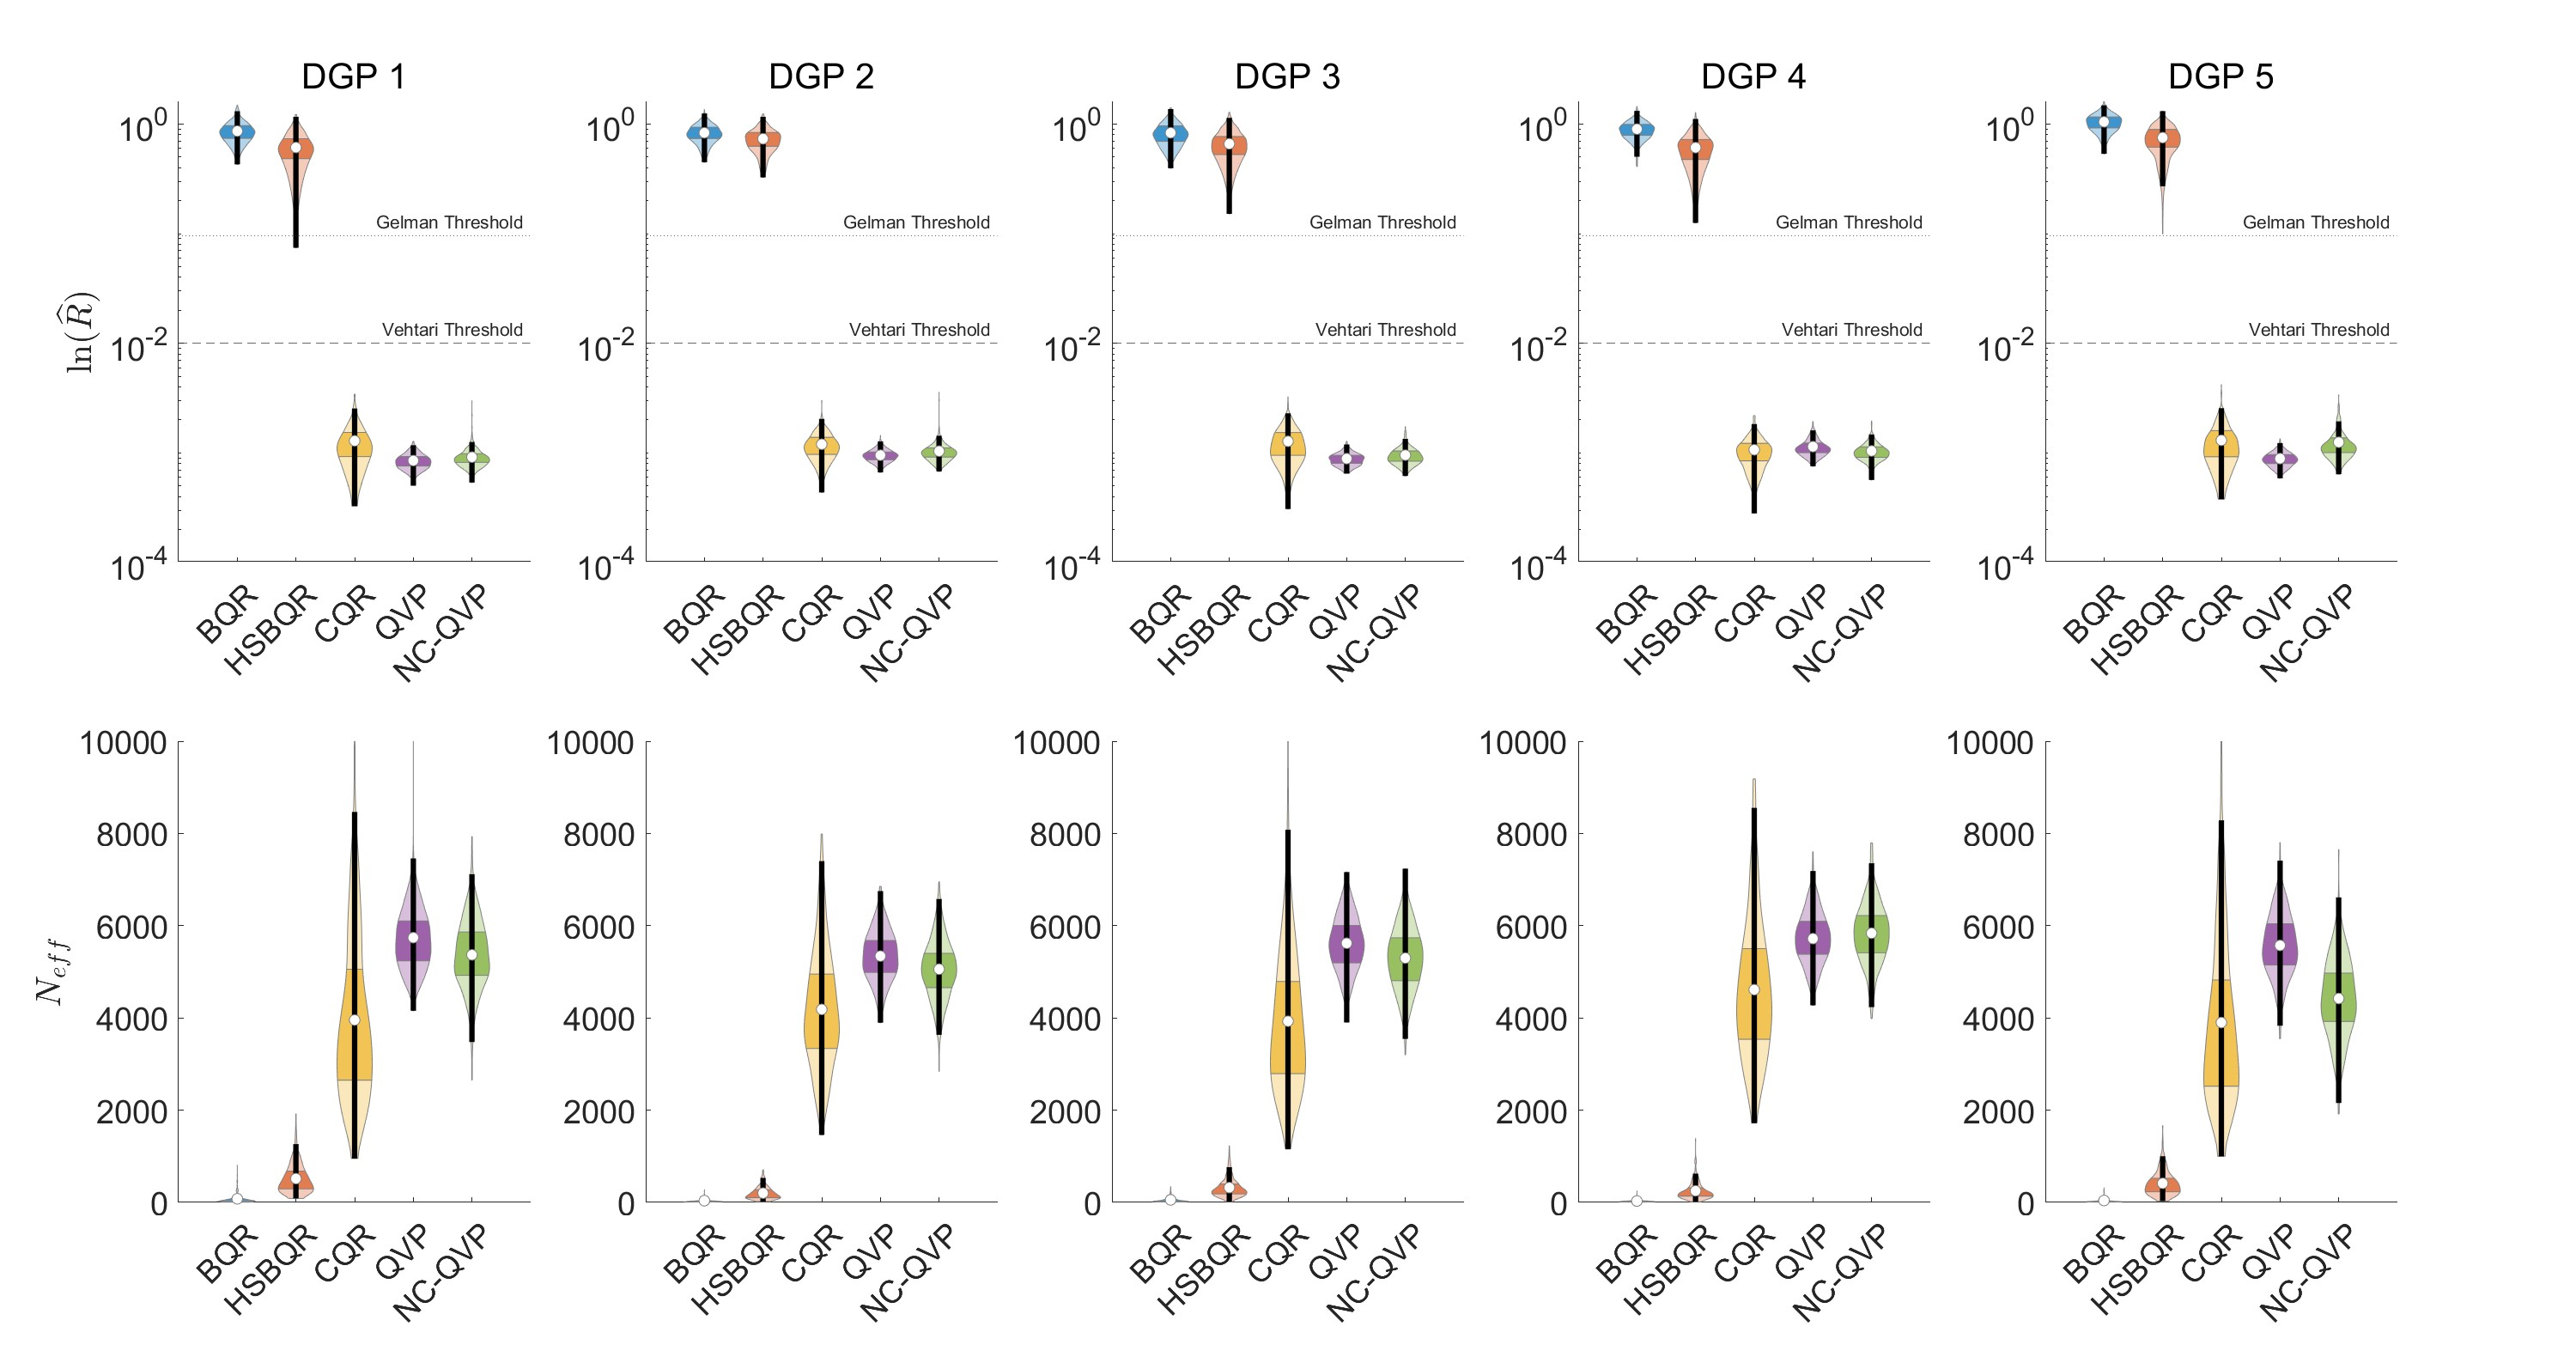
\includegraphics[width=\linewidth]{Figures/Robustness.jpg}
    \caption{Robustness measures ($\mathcal{T}=300$,$\varDelta$=0) $\hat{R}$ and $N_{\mathrm{eff}}$ are calculated according to \citet{vehtari2021rank} from 4 $\mathrm{MCMC}$ chains with 10k burnin and 15k saved draws. We indicate $\hat{R}$ thresholds according to \citet{vehtari_practical_2017} as well as \citet{gelman_bayesian_1996}.}
    \label{fig:RobustMeas}
\end{figure}
\vspace{-0.5cm}
%whisker plots or violin plots for Neff. For Rhat also a whisker plot or violin plot with a dashed line  on y axis showing the cutoff. Also have a set of panels focusing only the joint estim stuff. DO NOT SHOW SAVS VARIANTS SINCE THESE ARE BASED ON THE UNSPARSIFIED DRAWS!!


\begin{table}[]
\centering
%\resizebox{1\textwidth}{!}{%
\begin{tabular}{l|ccccc}
   & C1 & C2 & C3 & C4 & C5 \\ \hline
%$BRW$ & 0.00\% & 0.00\% & 0.00\% & 0.00\% & 0.00\% \\
%$CQR_{HS}$ & 0.00\% & 0.00\% & 0.00\% & 0.00\% & 0.00\% \\ \hdashline
$\BQR$ & 71.01\% & 75.17\% & 74.95\% & 72.86\% & 66.75\% \\
$\HSBQR$ & 34.24\% & 50.93\% & 44.06\% & 60.51\% & 35.72\% \\ \hdashline
$\QVP$ & 0.28\% & 0.11\% & 0.06\% & 1.22\% & 0.11\% \\
$\NCQVP$ & 0.06\% & 0.35\% & 0.17\% & 1.46\% & 0.28\% \\
$\NCQVP_{\mathrm{SAVS}}$ & 0.04\% & 0.11\% & 0.06\% & 1.35\% & 0.36\% \\ \hline
\end{tabular}%
%}
\caption{Crossing incidence (see Equation~\ref{eq:cross-i}) for $\mathcal{T}=300$,$\varDelta$=0. Estimates are based on the posterior mean of the coefficients.}
\label{tab:cross}
\end{table}

%\subsubsection{Coefficient profiles}
%Next we will look at the how the coefficient profiles look across the different monte carlo experiments. Ideally we want to have the true beta profile in the 1 standard deviation confidence band, with the mean coefficient profile being as close to the true beta profile as possible. We show $\beta_1$ for Case 1 in figure (\ref{fig:C1}), $\beta_5$ for Case 2 in figure (\ref{fig:C2}), $\beta_5$ for Case 4 in figure (\ref{fig:C4}), and $\beta_3$ for Case 5 in figure (\ref{fig:C5}).

%The quantile varying variable from Case 1 in figure (\ref{fig:C1}) shows a distinctive picture that all estimators seem to capture the quantile variation seeing how the true beta profile is within the confidence band for all the estimators. Having said that, the performance is not equal among the estimators. In particular, the BQR, CQR, and SAVS variant of the NCQVP have an average quantile profile that miss the quantile variation at the upper quantiles. However, the other NCQVP (and QVP) estimators perform much better, with quantile profiles very close to the true beta. Furthermore, when looking at the confidence bands, we can see that the estimators that jointly estimate the quantiles perform better, with tighter confidence bands. The NCQVP perform particularly well with mean profiles tracking the true beta profile closely, and confidence being tighter than the BRW estimator. Unsurprisingly, the CQR performs the worst, with an estimated profile of no quantile variation.

%The quantile constant variable in figure (\ref{fig:C2}) show again that jointly estimating the quantiles yields better performance. In particular we can see that these estimators have little to not quantile variation just like the true beta profile. Furthermore, the confidence bands of these estimators are tighter than that of the BQR and HSBQR. We can see in this figure that the SAVS variant is particularly potent having the confidence bands as tight as the CQR's which should perform the best for the quantile constant coefficients.

%The quantile specific sparse variable in figure (\ref{fig:C4}) shows how all the estimators have trouble with quantile specific sparsity. Surprisingly, the estimators that independently estimate the quantiles capture the quantile specific sparsity the least (apart from the CQR). Furthermore, at the tails, the true beta is outside the confidence intervals for these estimators. Of the joint estimation procedures we can see that the NCQVP and QVP has the best profile with average profiles being closest to the true beta profile. Furthermore the confidence intervals correctly show quantile variation around the tails only.


%The large quantile varying variable in figure (\ref{fig:C5}) show again how the joint estimation framework has advantages. In particular, we can see that, apart from the CQR, the BQR performs the worst and misses the true beta profile in the tails. The HSBQR performs better than the BQR but has relatively large confidence bands. The joint estimation methods capture the true beta profile better, with tighter confidence bands. %The only case where this is not true is the ASIS with SAVS, where the true beta profile is outside the confidence band at the central quantiles. 
%One interesting finding is that the SAVS variant overshrinks at the central quantiles, as can be seen by the average beta profiles. As such, for large quantile variation imposing SAVS can have negative consequences on the beta profiles. 

